%-------------------------------------------------------------------------------
%                                PREAMBLE
%-------------------------------------------------------------------------------
\documentclass[usenames,dvipsnames,svgnames,10pt,aspectratio=169]{beamer}
\usefonttheme{professionalfonts}

% This theme uses TIKZ: compile twice with PDFLaTeX or LuaLaTeX.
%
%  Options:
%  - [clean]:    clean slides, i.e. logos and footbar are removed
%  - [kth]:      footbar style inspierd to the official KTH template
%  - [nicewave]: a different style of wave is used (not approved by FLOW)
%
\usetheme{flow}

\usepackage{hyperref,graphicx,lmodern}
\usepackage[utf8]{inputenc}
\usepackage{media9}
\usepackage{xcolor}
\usepackage{stmaryrd}
\usepackage{nicefrac}
\usepackage{multimedia}
\usepackage{multicol}
\usepackage{upgreek}
\usepackage[]{bm}
\usepackage[]{url}

\graphicspath{{imgs/}}
\setbeamertemplate{blocks}[rounded][shadow=true]


%-------------------------------------------------------------------------------
%                                TITLE PAGE
%-------------------------------------------------------------------------------
\title[Nonlinear Physics] % Short title used in footline
{
	Nonlinear physics, dynamical \\ systems and chaos theory
}

\author[J.-Ch.~Loiseau] % Presenting author in short form used in footline
{
	Jean-Christophe Loiseau
}
% - Give the names in the same order as the appear in the paper.
% - Underline the presenting author.

\institute[unused]
{
	\url{jean-christophe.loiseau@ensam.eu} \\
	DynFluid, \\
	Arts et M\'etiers ParisTech, France
}
% Keep it simple, no one is interested in your street address.

% University logo(s)
\logot{
\includegraphics[width=.128\paperwidth]{DynFluid_logo}}  % Top logo
\logob{
\includegraphics[width=0.128\paperwidth]{ENSAM_logo}} % Bottom logo
% \logoc[{
\includegraphics[width=.128\paperwidth]{limsi}}]{
\includegraphics[width=.128\paperwidth]{limsi}} % Corner logo
%
% Cover image: \cvrimg{x position}{y position}{cover image}
\cvrimg{.77}{.8}{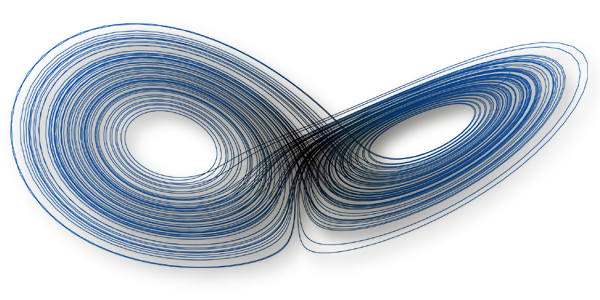
\includegraphics[width=.4\paperwidth]{cover.png}}

\date[unused]{ENSAM, Master 2, 2017--2018}

\begin{document}

\titleframe % Print the title as the first slide

%-------------------------------------------------------------------------------
%                           PRESENTATION SLIDES
%-------------------------------------------------------------------------------

\begin{frame}[t, c]{}
	\centering
	\vspace{1cm}

	{\Large \textbf{First-order systems}}

	\bigskip

	{\textgre{\textbf{Flows on the line}}}

\end{frame}

\begin{frame}[t, c]{First-order systems}{An apparently simple system}
	\begin{itemize}
		\item Let us consider the following first-order dynamical system
		$$
		\dot{x} = \sin(x).
		$$

		\bigskip

		\item Its analytical solution is given by
		$$
		t = \displaystyle \ln \left\vert \frac{\csc(x_0) + \cot(x_0)}{\csc(x) + \cot(x)} \right\vert.
		$$
	\end{itemize}

	\vspace{1cm}
\end{frame}

\begin{frame}[t, c]{First-order systems}{Phase line}
	\centering

	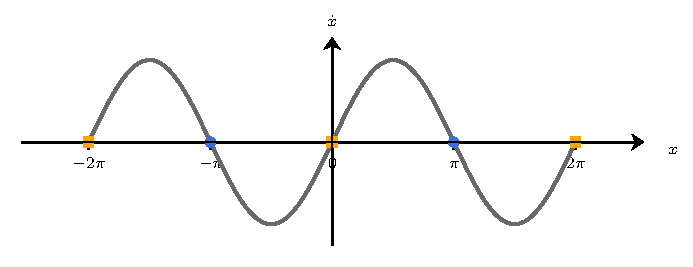
\includegraphics[width=.75\textwidth]{flow_on_the_line}

	\vspace{1cm}
\end{frame}

\begin{frame}[t, c]{First-order systems}{Fixed points}
	\begin{itemize}
		\item Fixed points $x^*$ are equilibrium solutions characterized by
		$$
		f(x^*) = 0.
		$$

		\bigskip

		\item In the present case, these are given by
		$$
		x^* = n \pi \text{ for } n \in \mathbb{N}.
		$$
	\end{itemize}

	\vspace{1cm}
\end{frame}

\begin{frame}[t, c]{First-order systems}{Linear stability}
	\begin{itemize}
		\item The dynamics of a perturbation $\eta(t) = x(t) - x^*$ is given by
		$$
		\dot{\eta} = f(x^* + \eta).
		$$

		\bigskip

		\item If $\eta$ is small enough, $f(x^* + \eta)$ can be approximated by its first-order Taylor expansion around $x^*$
		$$
		f(x^* + \eta) = f(x^*) + f^{\prime}(x^*) \eta + \mathcal{O}(\eta^2).
		$$
	\end{itemize}

	\vspace{1cm}
\end{frame}

\begin{frame}[t, c]{First-order systems}{Linear stability}
	\begin{itemize}
		\item Given that $f(x^*) = 0$, the dynamics of $\eta$ are governed by
		$$
		\dot{\eta} = f^{\prime}(x^*) \eta.
		$$

		\bigskip

		\item Its analytical solution is given by
		$$
		\eta(t) = \exp \left( f^{\prime}(x^*) t \right) \eta_0.
		$$
	\end{itemize}

	\vspace{1cm}
\end{frame}

\begin{frame}[t, c]{First-order systems}{Linear stability}
	\begin{itemize}
		\item The linear stability of a fixed point $x^*$ is determined by the sign of $f^{\prime}(x^*)$:

		\begin{itemize}
			\item[$\hookrightarrow$] if $f^{\prime}(x^*) > 0$, $\eta(t)$ growths exponentially fast. The fixed point is said to be \alert{\textbf{linearly unstable}}.

			\medskip

			\item[$\hookrightarrow$] if $f^{\prime}(x^*) < 0$, $\eta(t)$ decays exponentially fast. The fixed point is said to be \alert{\textbf{linearly stable}}.

			\medskip

			\item[$\hookrightarrow$] if $f^{\prime}(x^*) = 0$, one can not conclude and nonlinear analyses are required.
		\end{itemize}

		\bigskip

		\item Let us now re-analyze our original system and sketch the evolution of $x(t)$.
	\end{itemize}

	\vspace{1cm}
\end{frame}

\begin{frame}[t, c]{First-order systems}{Phase line}
	\centering

	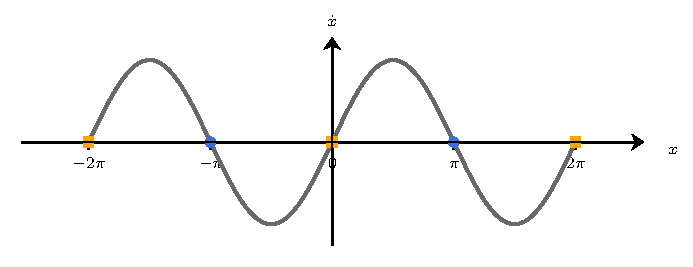
\includegraphics[width=.75\textwidth]{flow_on_the_line}

	\vspace{1cm}
\end{frame}

\begin{frame}[t, c]{First-order systems}{Evolution of $x(t)$}
	\centering

		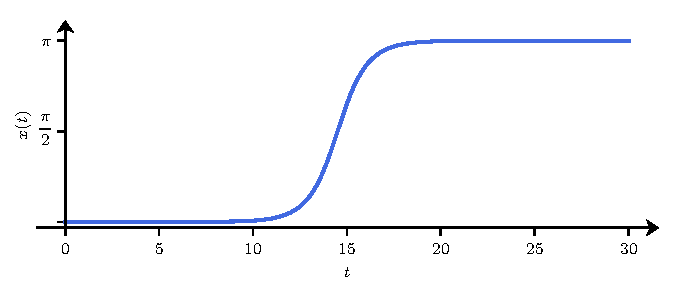
\includegraphics[width=.75\textwidth]{flow_on_the_line_bis}

	\vspace{1cm}
\end{frame}


\begin{frame}[t, c]{}
	\centering
	\vspace{1cm}

	{\Large \textbf{Second-order systems}}

	\bigskip

	{\textgre{\textbf{Oscillators, but not only...}}}

\end{frame}

\begin{frame}[t, c]{}{}

\end{frame}

\begin{frame}[t, c]{}
	\centering
	\vspace{1cm}

	{\Large \textbf{Interlude}}

	\bigskip

	{\textgre{\textbf{How to compute fixed points?}}}

\end{frame}

\begin{frame}[t, c]{How to compute fixed points?}{Different techniques}
	\begin{itemize}
		\item Fixed points are structuring the phase space of the dynamical system under scrutiny. Unfortunately, it may not be easy (nor possible) to compute them analytically.

		\bigskip

		\item A number of different numerical techniques exist for that purpose. The following list is by no means exhaustive:
		\begin{itemize}
			\item[$\hookrightarrow$] Newton-Raphson method,
			\item[$\hookrightarrow$] Selective Frequency Damping,
			\item[$\hookrightarrow$] BoostConv,
			\item[$\hookrightarrow$] ...
		\end{itemize}
	\end{itemize}

	\vspace{1cm}
\end{frame}

\begin{frame}[t, c]{Newton-Raphson method}{$f : \mathbb{R} \to \mathbb{R}$}

\end{frame}

\begin{frame}[t, c]{Newton-Raphson method}{$f : \mathbb{R} \to \mathbb{R}$}
	\begin{itemize}
		\item After $k$ iterations, the basic iteration scheme can be written as
		$$
		x_{k+1} = x_k - \displaystyle \frac{f(x_k)}{f^{\prime}(x_k)}.
		$$

		\bigskip

		\item Iteration stops when a user-defined criterion is fulfilled, usually
		$$
		\| f(x_k) \| \le \epsilon \text{ or } \| x_{k+1} - x_k \| \le \epsilon,
		$$
		with $\epsilon \simeq 10^{-10}$.
	\end{itemize}

	\vspace{1cm}
\end{frame}


\begin{frame}[t, c]{Newton-Raphson method}{$f : \mathbb{R} \to \mathbb{R}$}
	\centering

	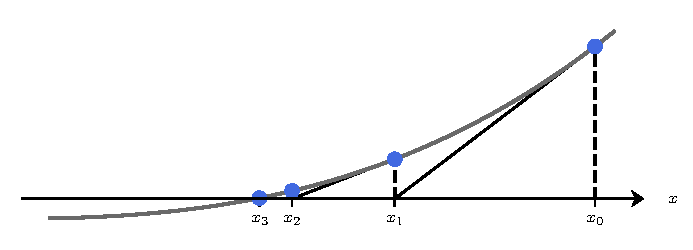
\includegraphics[width=.75\textwidth]{Newton_method}

	\bigskip

	Illustration of the Newton-Raphson for $f(x) = x^3 - 2x - 5$.

	\vspace{1cm}
\end{frame}


\begin{frame}[t, c]{Newton-Raphson method}{${\bm f} : \mathbb{R}^n \to \mathbb{R}^n$}

	\begin{itemize}
		\item Generalization of the Newton-Raphson method to the case ${\bm f} : \mathbb{R}^n \to \mathbb{R}^n$ is quite straightforward.

		\bigskip

		\item Given an estimate ${\bm x}_k$, the basic iteration reads
		\begin{equation}
			\begin{aligned}
				{\bm J} \delta {\bm x} & = - {\bm f}({\bm x}_k) \\
				{\bm x}_{k+1} & = {\bm x}_k + \delta {\bm x},
			\end{aligned}
			\notag
		\end{equation}
		where ${\bm J}$ is the Jacobian matrix of ${\bm f}$ evaluated at ${\bm x}_k$.
	\end{itemize}

	\vspace{1cm}
\end{frame}

\begin{frame}[t, c]{Newton-Raphson method}{${\bm f} : \mathbb{R}^n \to \mathbb{R}^n$}

\end{frame}

\begin{frame}[t, c]{Newton-Raphson method}{Limitations}
	\begin{itemize}
		\item Although efficient, Newton-Raphson method suffers from a number of limitations:
		\begin{itemize}
			\item[$\hookrightarrow$] The fixed points computed may depend on the initial guess ${\bm x}_0$.
			\item[$\hookrightarrow$] Evaluating ${\bm f}({\bm x})$ might be computationally expensive.
			\item[$\hookrightarrow$] At each iteration, the Jacobian matrix ${\bm J}$ needs to be evaluated and inverted ($\mathcal{O}(n^3)$ operations).
		\end{itemize}

		\bigskip

		\item A number of variants of the Newton-Raphson method exist as to address these different limitations. This however is algorithmic refinement beyond the scope of the present course.
	\end{itemize}

	\vspace{1cm}
\end{frame}

\end{document}
